% BLoC introduction
% What is the BLoC Pattern
% What is a single BLoC
% How is BLoC implemented in The Giraf project
% What are the Giraf Project guidelines regarding BLoCs
\section{BLoC Pattern}
When we moved the application to Flutter, we chose to structure the code with the \gls{bloc} pattern. The following chapter describes this pattern.

The name \gls{bloc} is used for two things, the \gls{bloc} pattern and classes called \glspl{bloc}. To avoid confusion we always write \gls{bloc} pattern when we refer to the pattern. In all other cases we refer to the classes.

\subsection{Background}
\gls{bloc} is a pattern that aims to isolate all business logic from \gls{ui} code \cite{blocPattern}. Paolo Soares designed the pattern while he worked on the Google platform; AdWords \cite[30 sec]{blocPattern}. Paolo Soares presented the \gls{bloc} pattern at DartConf 2018 in a speach called "Code sharing, better together" \cite{blocPattern}.
The background for the \gls{bloc} pattern is that the Google AdWords team  developed two applications; a web-application and a mobile application \cite[30 sec]{blocPattern}.
They developed the applications before Flutter existed, and had to make native code bases, for iOS and Android, for the mobile application, as well as one for the web application \cite[30 sec]{blocPattern}.
Because they had three separate code bases, they had to maintain all three bases and repeat all changes three times \cite[30 sec]{blocPattern}.

When Flutter was released Paolo Soares, saw the possibility to merge the mobile-applications into one code base and thereby to achieve only one language for the development \cite[1 min 15 sec]{blocPattern}. They also initially thought that they would be able to reuse all the dart written business logic from the web-application and thereby very rapidly develop the mobile application \cite[1 min 48 sec]{blocPattern}. Trying to do so highlighted a considerable issue in their web-application which was that the business logic where mixed in with the \gls{ui} logic \cite[2 min 12 sec]{blocPattern}.

In order to re-use the business logic from the web-application they needed to separate business and \gls{ui} logic. The business logic had to be platform independent, meaning useable on both the web-application and the mobile-application without any modifications\cite[2 min 12 sec]{blocPattern}. This resulted in a pattern named \gls{bloc}.

\subsection{What is BLoC} \label{subsec:what_is_bloc}
To understand the \gls{bloc} pattern one first needs to understand what a \gls{bloc} is. A \gls{bloc} is a simple class that only takes sinks as input and exposes streams as output \cite[21 min 25 sec]{blocPattern}. All business logic should be inside a \gls{bloc}. The intuition is that \glspl{bloc} are the building blocks of the application \cite[21 min 25 sec]{blocPattern}. Another key requirement of a \gls{bloc} is that all depedencies should be injected \cite[22 min 55 sec]{blocPattern}, so if an api is needed it should be injected in the constructor of the \gls{bloc}. This allows the web-platform to use a JSON-API and the mobile-platform to use a BINARY-API and other simmilar situations, while all platforms still uses the same \glspl{bloc} without any modifications. An application thereby consist of many \glspl{bloc} with different responsibilities. The \glspl{bloc} can then be used by the \gls{ui} components of all platforms.

\subsubsection{Sinks and streams}
A \gls{bloc} can only communicate via sinks or streams\ref{subsec:what_is_bloc}. Both sinks and streams work as streams, but a sink is an input stream while a stream is for outputs.

A stream is an asynchronous sequence of data, similar to an asynchronous Iterable, but instead of the subscriber requesting the next item, the stream will emit as soon as a new item is ready \cite{dartStreams}. This means that a \gls{bloc} recieves data from the \gls{ui} via a sink and emits data via the stream, both asynchronous. Both the \gls{ui} component and the \glspl{bloc} will react instantaneously when ever new data is recieved.

This uncovers a requirement of the \gls{ui} component, which is state management. The \gls{ui} should not be required to rely on state building, since the \gls{bloc} streams are asynchronous, which is why the \gls{ui} components has to be able to handle streams \cite[4 min 40 sec \& 14min 00 sec]{blocPattern}.

\subsection{Rules of BLoC Pattern}
\begin{figure}[h]
    \centering
    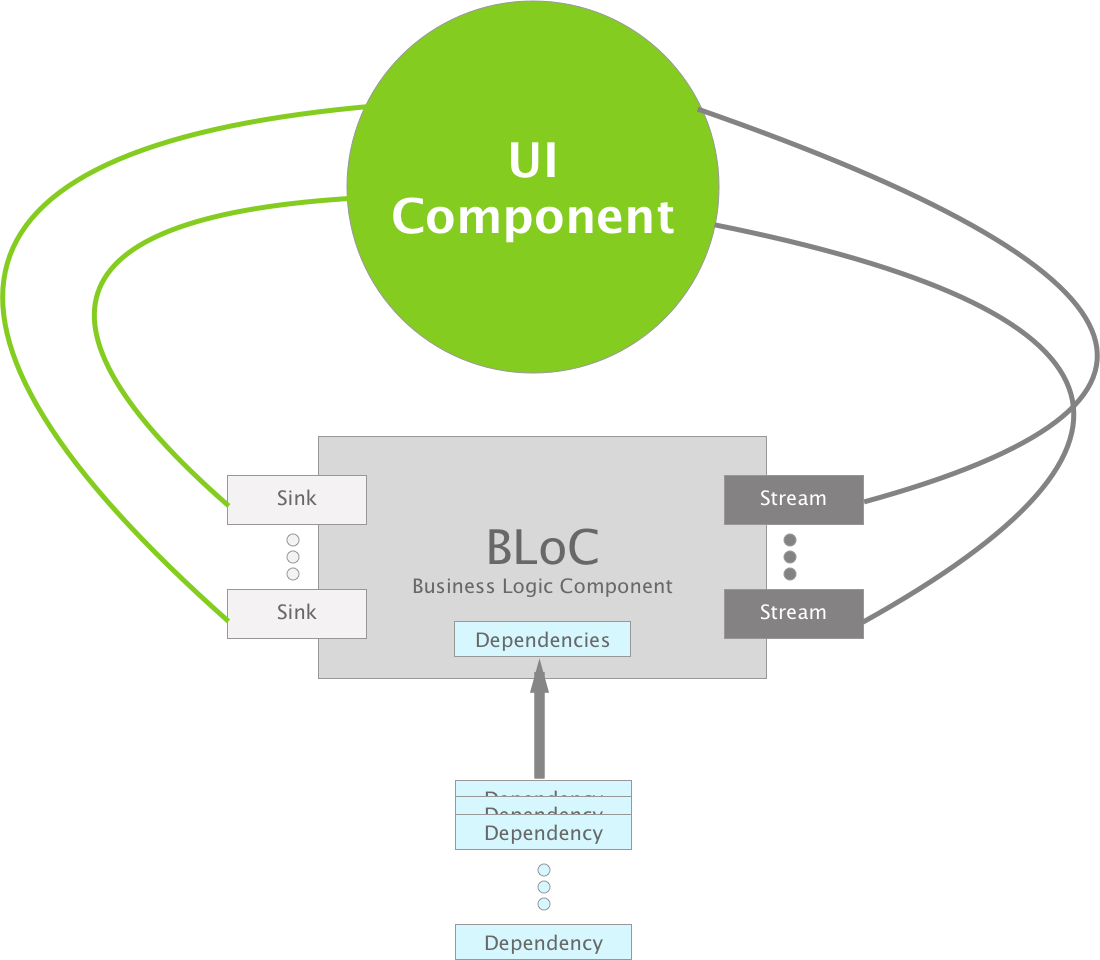
\includegraphics[width=0.8\textwidth]{figures/BLoCPattern.png}
    \caption{A illustration of the BLoC Pattern}
    \label{fig:blocPattern}
\end{figure}

The \gls{bloc} pattern can be boiled down to a set of rules and one practice. The practice is that the business and \gls{ui} logic should be clearly separated, with all the business logic inside a specific \glspl{bloc}. An application should have multiple \glspl{bloc}. The decision of how to divide the business logic into multiple \glspl{bloc} is a judgement call. As Paolo Soares puts it "each complex enough component has its own BLoC" \cite[24 min 15 sec]{blocPattern}. The rules of the \gls{bloc} pattern are listed in the following text as presented by Paolo Soares \cite[22 min 25 sec]{blocPattern}.

There are some guidelines for the design of \glspl{bloc} that have to be upheld when the \gls{bloc} pattern is used.
\begin{itemize}
  \item Inputs and outputs are simple Streams/Sinks only
  \item Dependencies must be injectable and platform agnostic
  \item No platform branching allowed
  \item Implementation can be whatever you want if you follow the previous rules
\end{itemize}

The first rule states that any communication between the \gls{ui} and a \gls{bloc} must be through Sinks and Streams, so when the \gls{ui} should send data to the \gls{bloc} it should use a sink, and when a \gls{bloc} sends data to the \gls{ui} it should use a stream.

The second rule states that all dependencies of a \gls{bloc} must be injectable; this is crucial for platform independence since it is makes it possible to inject the correct dependencies for each platforms.


The third rule states that it is not allowed to branch depending on the platform, meaning the business logic should be completely independent of the platform. What the rule is effectively stating is that inside a \gls{bloc} there should not be e.x., an if-statement checking if the platform is iOS and do some computation on behalf of that.

The last rule states that the \gls{bloc} pattern can be implemented however the developer finds appropriate, as long as the other rules are upheld. Therefore the pattern is flexible and can be used in many different cases.

The following rules should be followed during the design of the \gls{ui}.
\begin{itemize}
  \item Each "Complex enough" component has a corresponding \gls{bloc}
  \item Components should send inputs "as is"
  \item Components should show outputs as close as possible to "as is"
  \item All branching should be based on simple \gls{bloc} Boolean outputs
\end{itemize}

The first rule states that if the \gls{ui} component is complex enough it should have its own \gls{bloc}, thereby also stating that \gls{ui} components should share \glspl{bloc} if they are non-complex.

The second rule states that if the \gls{ui} needs to send data to the \gls{bloc}, i.e., User inputs, the \gls{ui} component is not allowed to do any computation on the inputs before sending it to the \gls{bloc}; this is a step to ensure decoupling between the \gls{ui} and Business logic.

The third rule is much like the second but concerns output instead of input. The output from a \gls{bloc} should not be changed inside the \gls{ui} component, this again is to ensure that all business logic stays inside the \gls{bloc}.

The fourth rule states that all business logic dependent if-statements inside the \gls{ui} component should only depend on one boolean stream from the \gls{bloc}, this again is to decouple the \gls{ui} component from the business logic, since branching on business logic in the \gls{ui} most likely would hard couple \gls{ui} and business logic.

\subsection{BLoC Implementation in the Giraf Project}
The Flutter framework is not opinionated towards which architecture should be used so we had to decide for ourselves. We chose the \gls{bloc} pattern after considering other patterns like MVVM and MVC. In order to compare the different patterns, we made some goals we wanted the pattern to fulfil. This enabled us to compare the different patterns to each other and find the one that best fitted our needs. The goals were:

\begin{itemize}
  \item Business logic should be re-useable by all widgets
  \item There should be a clear seperation between \gls{ui} and business logic.
  \item \gls{ui} components should be reactively, ie. if data changes in one component then the change should automaticly be reflected in all other components relying on the same data.
  \item The pattern should allow for a intuitive file structure.
\end{itemize}

Doing some empirical experiments in building with the different patterns and reading different developers experience with the different patterns we came to the conclusion that the \gls{bloc} pattern offered the most freedom while still isolating the business logic and \gls{ui} logic. The \gls{bloc} pattern also allow for all the other goals. Because of this and the fact that we only had 3 days to complete the rebuild, we decided to use the \gls{bloc} pattern.

Because there is a large degree of freedom, we had to find out how we should use the pattern in the project. We did some research on how people in the \gls{bloc} community used it. We found that rxDart was a favourite library for \gls{bloc} implementation. In our experience it can be a good idea to follow the community since there exists many great resources on how to use it and popular libraries are less likely to be abandoned. Therefore we decided to use this library.

\subsubsection{rxDart}
"RxDart is a reactive functional programming library for Google Dart, based on ReactiveX." \cite{rxDart}. The Dart Language has a decent Stream support, rxDart uses this to add the ReactiveX functionality on top of the native stream api \cite{rxDart}. To better understand how it helps in implementing the \gls{bloc} pattern we will provide a short explanation of what ReactiveX is and describe the key features from the rxDart library that are used in the Giraf Project.

ReactiveX is a library in which one can use observable sequences to create asynchronous and event-based programs, "It extends the observer pattern to support sequences of data and/or events and adds operators that allow you to compose sequences together declaratively while abstracting away concerns about things like low-level threading, synchronization, thread-safety, concurrent data structures, and non-blocking I/O." \cite{ReactiveXWebsite}.

The main features used from the rxDart library are three different stream behaviours, which are PublishSubject, BehaviorSubject and ReplaySubject. With these three stream behaviours, or subjects as rxDart refers to them, it is possible to implement any desired functionality.

\subsubsection*{PublishSubject}
\begin{figure}[h]
    \centering
    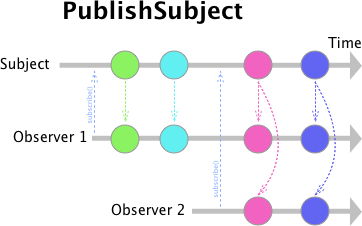
\includegraphics[width=0.8\textwidth]{figures/PublishSubject.png}
    \caption{A illustration of the behavior of a PublishSubject}
    \label{fig:PublishSubject}
\end{figure}
The PublishSubject behaves like the Dart Lang native StreamController, but with one exception, which is; a PublishSubject returns a Observable, where a StreamController returns a stream \cite{PublishSubject}. This means that the PublishSubject upholds the ReactiveX Subject contract and there by allow for all the ReactiveX operations \cite{PublishSubject}. The behaviour of a PublishSubject across time is shown in \autoref{fig:PublishSubject}.

\subsubsection*{BehaviorSubject}
\begin{figure}[h]
    \centering
    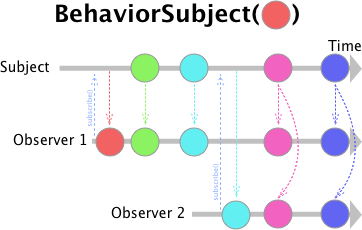
\includegraphics[width=0.8\textwidth]{figures/BehaviorSubject.png}
    \caption{A illustration of the behavior of a BehaviorSubject}
    \label{fig:BehaviorSubject}
\end{figure}
The BehaviorSubject behaves similar to the PublishSubject, but with one exception, it captures the latest item that has been added to the subject and emits that as the first item every time a new observer subscribes \cite{BehaviorSubject}. The BehaviorSubject can also be seeded with a initial item, that will be the first item emitted in case no items has been added to the subject yet. The behaviour of a BehaviorSubject across time is shown in \autoref{fig:BehaviorSubject}.

\subsubsection*{ReplaySubject}
\begin{figure}[h]
    \centering
    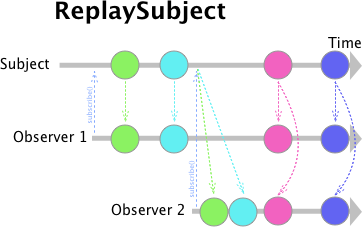
\includegraphics[width=0.8\textwidth]{figures/ReplaySubject.png}
    \caption{A illustration of the behavior of a ReplaySubject}
    \label{fig:ReplaySubject}
\end{figure}
The ReplaySubject behaves similar to the BehaviorSubject, but instead of only capturing the latest item, it captures all items and emits them whenever a new observer subscribes \cite{ReplaySubject}. Unlike the BehaviorSubject, the ReplaySubject can not be seeded with an initial value. The behaviour of a ReplaySubject across time is shown in \autoref{fig:ReplaySubject}

\subsection{BLoC Design Guidelines of the Giraf Project}
The Giraf Project have altered the rules of the \gls{bloc} pattern a bit. The reason for this is that in the Giraf Project we are not using the code in other platforms than the Flutter Framework, therefore to make the use of \glspl{bloc} a bit more intuitive and flexible for the developers we have constructed the following design guideline:

\subsubsection{Giraf Project BLoC Pattern Guidelines}
\begin{itemize}
  \item Rather many small non-complex \glspl{bloc} than few large complex \glspl{bloc}
  \item Start by creating a \gls{bloc} per \gls{ui} Screen, then after implementing the functionality consider to refactor to shared \glspl{bloc}
  \item Inputs to \glspl{bloc} should be either Sinks or function calls with parameters
  \item \glspl{bloc} should be instantiated via the dependency injector/ Thereby all dependencies should also be injectable
  \item \glspl{bloc} are to be implemented using the rxDart library
\end{itemize}


